\section{Theorie}
\label{sec:Theorie}

Die Milikan-Methode zur Bestimmung der Elementarladung basiert auf der Zerstäubung von Öltröpfchen in das elektrische Feld eines Plattenkondensators. 
Durch die Reibung der Tröpfchen mit der Luft werden sie elektrisch geladen. Die Ladung $q$ der Tröpfchen kann nur ein ganzzahliges Vielfaches der 
Elementarladung sein. Das elektrische Feld des Plattenkondensators ist vertikal ausgerichtet, wodurch die auf die geladenen Teilchen wirkende 
elektrische Kraft $\vec{F}_\text{el}$ parallel oder antiparallel zur Gravitationskraft $\vec{F}_\text{g}$ wirkt. Zusätzlich wirkt die Stokesche 
Reibungskraft $\vec{F}_\text{R}$ entgegen der Bewegungsrichtung, da sich die Teilchen mit einer Geschwindigkeit $\vec{v}$ durch den luftgefüllten 
Raum bewegen.

Die Wirkung dieser Kräfte auf ein Teilchen kann durch folgende Gleichungen beschrieben werden:

\begin{align}
    \label{eqn:Kraefte}
    \vec{F}_\text{g} &= m \vec{g} \\
    \vec{F}_\text{el} &= q \vec{E} \\
    \vec{F}_\text{R} &= -6\symup{\pi}r\eta_\text{L} \vec{v}
\end{align}

Hierbei steht $m$ für die Masse des Teilchens, $\vec{g}$ für die Fallbeschleunigung, $\eta_\text{L}$ für die Viskosität der Luft und $r$ für den Radius 
des Teilchens.

Nach einer kurzen Zeit stellt sich ein Kräftegleichgewicht ein, bei dem sich die Tröpfchen mit konstanter Geschwindigkeit bewegen. Bei abgeschaltetem 
elektrischen Feld bewegen sich die Öltröpfchen mit der Geschwindigkeit $v_0$ und erhalten durch den Auftrieb der Luft den Radius:

\begin{equation}
    \label{eqn:Radius}
    r = \sqrt{\frac{9 \eta_\text{L}(v_\text{ab} - v_\text{auf})}{4g(\rho_\text{Oel}- \rho_\text{L})}}.
\end{equation}

Das Kräftegleichgewicht führt zu folgender Gleichung:

\begin{equation*}
    \frac{4\symup{\pi}}{3}r^3(\rho_\text{Oel}- \rho_\text{L})g = 6 \symup{\pi} \eta_\text{L}r v_0.
\end{equation*}

Abhängig von der Polung des elektrischen Feldes wirken die elektrostatische Kraft und die Reibungskraft in verschiedene Richtungen. Die Orientierung 
der Kräfte kann der Abbildung \ref{fig:Kraeftegleichgewicht} entnommen werden.

\begin{figure}
    \centering
    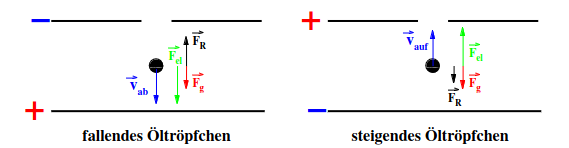
\includegraphics[width = .9\textwidth]{Bilder/Kraeftegleichgewicht.png}
    \caption{Orientierung der wirkenden Kräfte bei unterschiedlicher Polung des elektrischen Feldes. \cite{1}}
    \label{fig:Kraeftegleichgewicht}
\end{figure}

Wenn die obere Platte des Kondensators positiv geladen ist und eine ausreichend große Spannung anliegt, bewegt sich das Öltröpfchen mit der 
Geschwindigkeit $v_\text{auf}$ nach oben. Das Kräftegleichgewicht ergibt sich zu:

\begin{equation*}
    \label{eqn:Kraefte_1}
    \frac{4\symup{\pi}}{3}r^3(\rho_\text{Oel} - \rho_\text{L})g + 6 \symup{\pi} \eta_\text{L}r v_\text{auf} = qE.
\end{equation*}

Bei entgegengesetzter Polung des elektrischen Feldes ergibt sich:

\begin{equation*}
    \label{eqn:Kraefte_2}
    \frac{4\symup{\pi}}{3}r^3(\rho_\text{Oel}- \rho_\text{L})g - 6 \symup{\pi} \eta_\text{L}r v_{\text{ab}} = -qE,
\end{equation*}

wobei $v_{\text{ab}}$ die nach unten gerichtete Geschwindigkeit ist.

Aus diesen beiden Gleichungen kann die Ladung $q$ des Öltröpfchens bestimmt werden:

\begin{equation}
    \label{eqn:q}
    q = \frac{9}{2} \symup{\pi} \sqrt{\frac{\eta_\text{L}^3(v_\text{ab} - v_\text{auf})}{g(\rho_\text{Oel}- \rho_\text{L})}} \cdot \frac{v_\text{ab} + v_\text{auf}}{E},
\end{equation}

wobei $E$ den Betrag des elektrischen Feldes darstellt. Die Geschwindigkeiten sind durch folgenden Zusammenhang gegeben:

\begin{equation}
    \label{eqn:v_0}
    2v_0 = v_\text{ab} - v_\text{auf}.
\end{equation}

Bei diesen Gleichungen \ref{eqn:q} muss eine Korrektur durchgeführt werden, weil die Gleichungen nur für Tröpfchen gelten deren Abmessungen größer 
als die mittlere freie Weglänge in Luft ist.
Die Korrektur ist dabei gegeben als
\begin{align}
\label{eq:Theorie_Cunningham_Viskositaet}
\eta_\text{eff}=\eta_\text{L}\left( \frac{1}{1+B\frac{1}{pr}} \right),
\end{align}
sie wird als \textbf{Cunningham-Korrekturterm} bezeichnet. 
Dazu wird der Luftdruck $p$ und die experimentell bestimmbare Konstante $B =  \num{6.17e-3}\, \text{Torr}\cdot\unit{\centi\metre}$ \cite{1} verwendet.
Es gilt $1\,\text{Torr} \approx \qty{133.322}{\pascal}$ \cite{2}.
Für die korrigierte Ladung gilt
\begin{equation}
    \label{eqn:q_korrigiert}
    q_\text{real} = q_0 \left(1+ \frac{B}{pr}\right)^{-3/2}.
\end{equation}